\chapter{Introduction}
\begin{quote}
Mathematics began to seem too much like puzzle solving. Physics is puzzle solving, too, but of puzzles created by nature, not by the mind of man.
\end{quote}
\begin{flushright}
--Maria Goeppert-Mayer
\end{flushright}

In the 18$^\textrm{th}$ century, Isaac Newton,  watching an apple fall to the ground, thought to himself, ``Why should that apple always descend perpendicularly to the ground?''
In short, why were there not other ways for apples to fall? While it would be significantly more difficult for apple trees to reproduce if they fell upwards, there surely had to be an explanation for why they would only fall downwards!
These musings led him to develop his theory on gravitation which not only describes how apples fall, but also describes the motion of the planets in the solar system.
Similarly, even as modern physics has tackled tougher problems than that of the motion of an apple to the ground, the underlying question is always the same: ``Why do things act a certain way?''
The answers found not only describe the ``apples" we are looking at, but the universe as a whole.

One way that this current question manifests to physicists now is ``Do neutrino particles act like other leptons?''
This indeed is the main question addressed in this thesis, and has been a topic of active study for nearly a century.

\section{The Standard Model}
\subsection{Overview}
Since the days of Newton, physics has come a long way in describing the fundamental building blocks of nature.
Currently, a theory developed in the 1960's known as the Standard Model of particle physics is the main explanation for physical phenomena and has correctly predicted the existence of multiple particles, most recently the Higgs boson \cite{Aad:2012tfa}\cite{Chatrchyan:2012xdj}.
The Standard Model is one of the most powerful theories in physics, and together with $\Lambda$CDM in cosmology, has been able to correctly predict phenomena on both subatomic and cosmological scales.

The Standard Model divides up the universe into two main types of particles: the particles that make up the matter around us, called fermions, and the particles that mediate the fundamental forces of nature, called bosons.
This splitting comes from the spins of the particles, viz., as the spins of fermions only come in half-integers, e.g. $\frac{1}{2}$, and the bosons are integers, e.g. 0 and 1.
The classifications can be further broken down for the fermions into two more sub-types of particles: quarks and leptons.
The full list of the fermions and bosons in the Standard Model is shown in \autoref{fig:StandardModel}, but the Standard Model does more than merely classify these particles found in nature, it also describes how each of these quarks and leptons interact with one another via the gauge bosons.
In particular, each of the gauge bosons -- the photon, the Z and W bosons, and the gluon -- correspond to one of the fundamental forces of nature: electromagnetic, weak nuclear force, and strong nuclear force, respectively.
The Higgs boson, while also a boson, does not mediate a force, but instead arises due to the spontaneous symmetry breaking of the electroweak force. 

\begin{figure}[tbph]
\centering
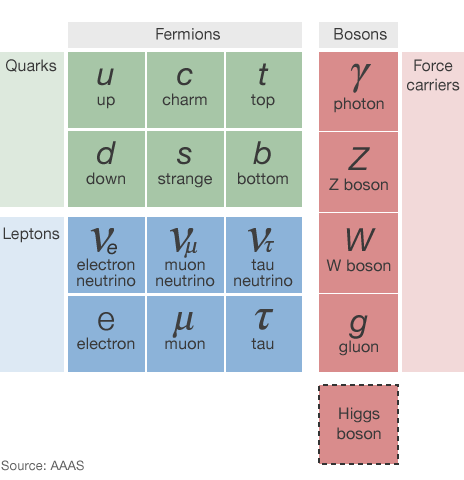
\includegraphics[width=0.6\linewidth]{Figures/higgs-elementary-particles.png}
\caption[The particles in the Standard Model]{The particles in the Standard Model. They are split into the bosons and fermions, with the fermions being further split into three generations of quarks and leptons.}
\label{fig:StandardModel}
\end{figure}

\subsection{Leptons}
Of greatest interest here for the work in this thesis are the particles, or flavors, known as leptons.
These 6 flavors are the electron, the muon, and the tau and the electron neutrino, the muon neutrino, and the tau neutrino.
These particles interact with one another via the W and Z bosons which is discussed in more detail in \autoref{sec:Beta Decay}. 
When the Standard Model was first introduced in the 1960's, the neutrinos were massless.
This was due to the fact that, as shown in \autoref{fig:NeutrinoMasses}, the masses of neutrinos are at least a million times lighter than the next-lightest particle, the electron with mass $0.511 \textrm{MeV}$
\footnote{Natural units, e.g. $c=1$ and $\hbar=1$, will be used throughout this thesis.
In this way, masses (units $\textrm{eV}/\textrm{c}^2$) and temperatures will be expressed in terms of energy, $\textrm{eV}$. 
Later on in the thesis, SI units will also be used, but the context of the units will make the convention clear.}.

\begin{figure}[tbph]
\centering
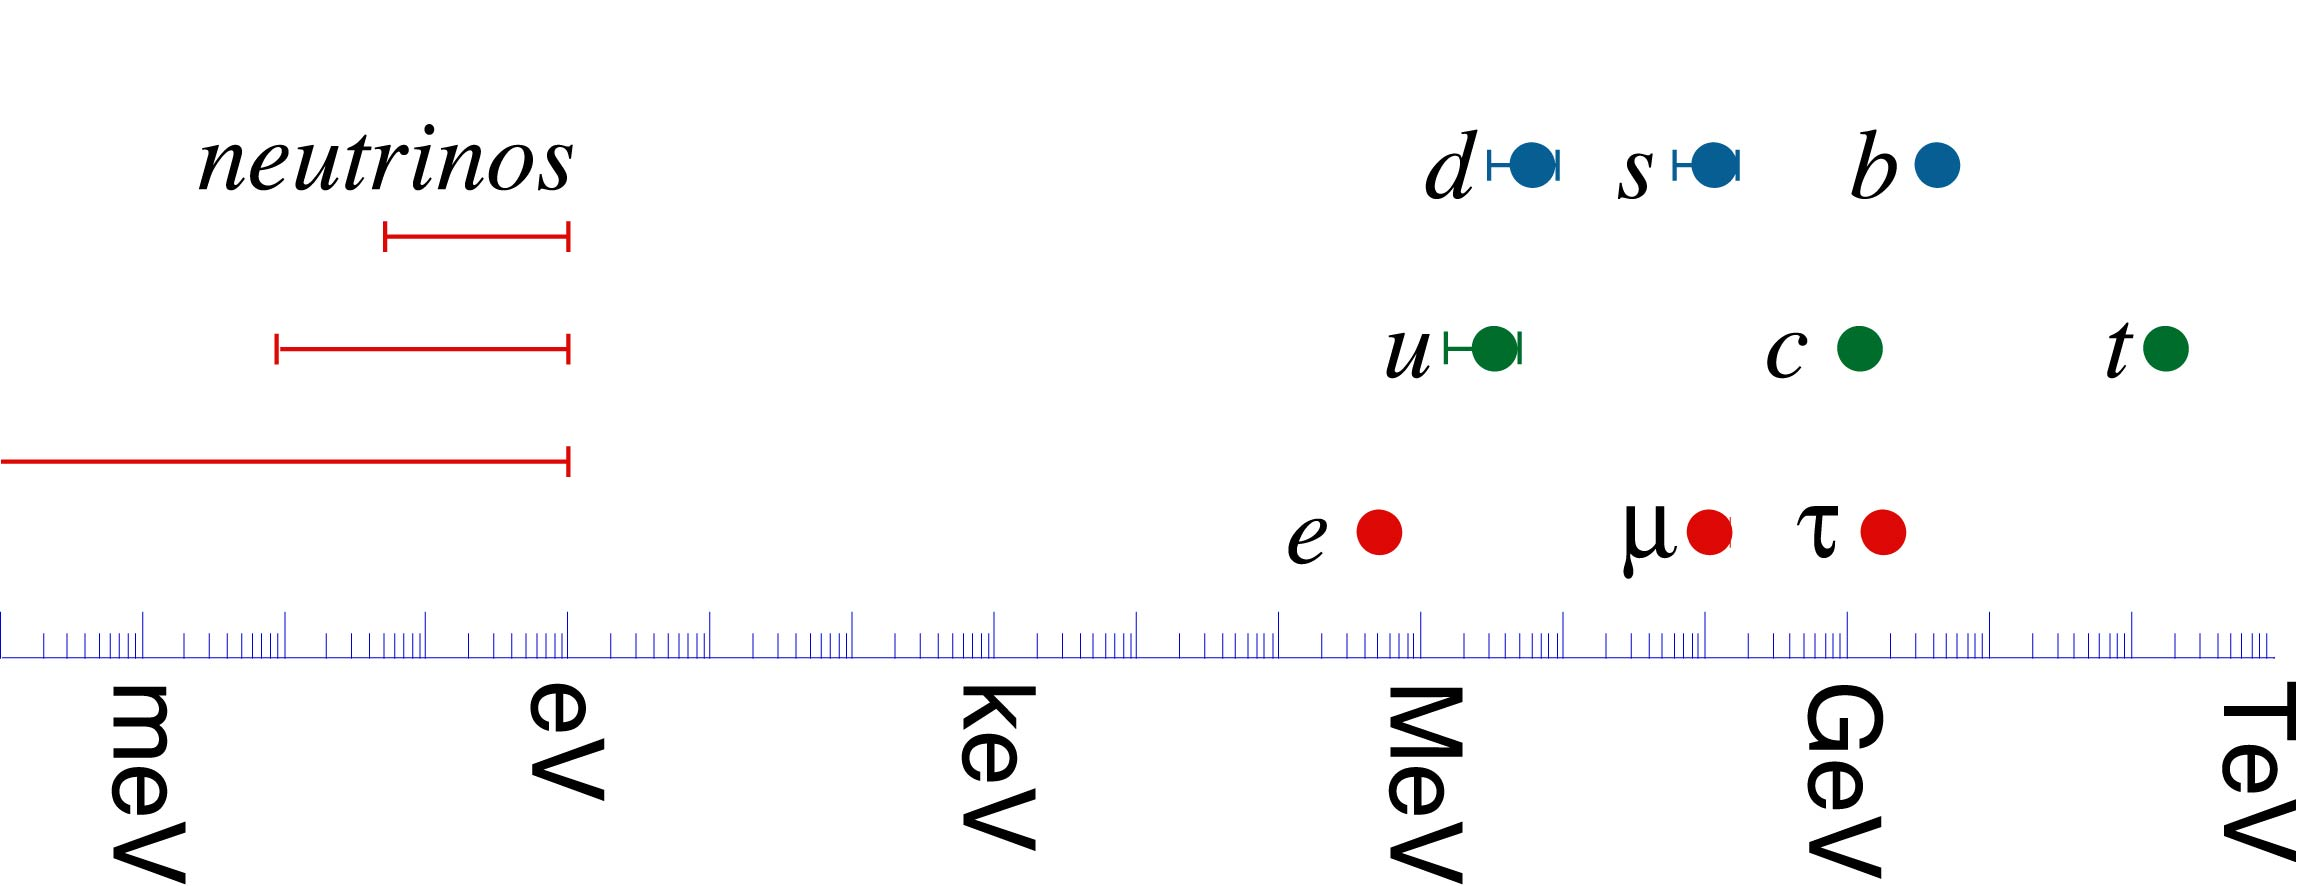
\includegraphics[width=0.9\linewidth]{Figures/NeutrinoMasses.jpg}
\caption[The masses of the fundamental fermion particles.
The neutrinos are multiple orders of magnitude lighter than even their lightest counterparts.]
{The masses of the fundamental fermion particles.
The neutrinos are multiple orders of magnitude lighter than even their lightest counterparts.}
\label{fig:NeutrinoMasses}
\end{figure}

\subsubsection*{Neutrino Masses and Oscillation}
\label{ssec:NeutrinoMassesandOscillation}
Neutrinos were shown to have mass, however, after they were observed to oscillate between their generational counterparts, viz. $\nu_{\textrm{\alpha}} \leftrightarrow \nu_{\textrm{\beta}}$, where $\alpha$ and $\beta$ correspond to two different flavor states of the neutrino \cite{PhysRevLett.20.1205}\cite{Hatakeyama:1998ea}\cite{Ahmad:2001an}.
Not only does this phenomenon imply that the neutrinos have non-zero mass, it also shows that the neutrino flavor eigenstates are not equivalent to their mass eigenstates.
This transformation between the flavor and mass bases can be represented as a matrix, called the Pontecorvo–-Maki–-Nakagawa–-Sakata (PMNS) matrix as follows:

\begin{equation}\label{eq:PMNS Matrix U Form}
\begin{bmatrix}
\nu_{e} \\
\nu_{\mu} \\
\nu_{\tau}
\end{bmatrix}
=
  \begin{bmatrix}
    U_{e1} & U_{e2} & U_{e3} \\
    U_{\mu1} & U_{\mu2} & U_{\mu3} \\
    U_{\tau1} & U_{\tau2} & U_{\tau3}
  \end{bmatrix}
  \begin{bmatrix}
  	\nu_{1} \\
	\nu_{2} \\
	\nu_{3}
  \end{bmatrix}.
  \end{equation}

In this formalism, the probability for measuring an electron neutrino to have the mass associated with the $\nu_1$ state is $|U_{e1}|^2$. The notation usually used to differentiate the $\nu_1$, $\nu_2$, and $\nu_3$ states is in decreasing order of the probability for a $\nu_i$ state to be observed in a $\nu_e$ state.
These probabilities are shown in \autoref{fig:Oscillations_electron_long}.
The PMNS matrix in \autoref{eq:PMNS Matrix U Form} can also be written as follows: 
\begin{equation}\label{eq:PMNS Matrix Standard Form}
  \begin{bmatrix}
    1 & 0 & 0 \\
    0 & c_{23} & s_{23} \\
    0 & -s_{23} & c_{23}
  \end{bmatrix}
  \begin{bmatrix}
  c_{13} & 0 & s_{13}e^{-i\delta_{CP}} \\
  0 & 1 & 0 \\
  -s_{13}e^{i\delta_{CP}} & 0 & c_{13}
  \end{bmatrix}
  \begin{bmatrix}
  c_{12} & s_{12} & 0 \\
  -s_{12} & c_{12} & 0 \\
  0 & 0 & 1
  \end{bmatrix}
  \begin{bmatrix}
  e^{i\alpha_1/2} & 0 & 0 \\
  0 & e^{i\alpha_2/2} & 0 \\
  0 & 0 & 1
  \end{bmatrix}
\end{equation}
where $s_{ij}$ and $c_{ij}$ are $\sin(\theta_{ij})$ and $\cos(\theta_{ij})$, respectively.
While this formulation in \autoref{eq:PMNS Matrix Standard Form} looks more complicated than the formulation in \autoref{eq:PMNS Matrix U Form}, it reduces the total number of parameters to just three mixing angles and a complex phase ($\theta_{12}$, $\theta_{13}$, $\theta_{23}$, and $\delta_{CP}$, respectively) due to the fact that five of these parameters can be absorbed into the phases of the lepton fields \cite{Valle:2006}.
The other parameters, $\alpha_1$ and $\alpha_2$, only play a role if the neutrino is a Majorana particle, which is discussed more in \autoref{ssec:Dirac and Majorana Masses}.
In any case, these values for $\alpha_1$ and $\alpha_2$ do not play a role in neutrino oscillation and their matrix can be thought of as the identity matrix in this scenario \cite{BILENKY1980495}.
To understand what this means for the behavior of neutrinos, a simpler model with only two neutrinos can be used.
In this simplified model with two neutrinos of flavor $\alpha$ and $\beta$, the usefulness of these angles and phases becomes apparent as \autoref{eq:PMNS Matrix Standard Form} appears as
\begin{equation}
\begin{bmatrix}
\nu_\alpha \\
\nu_\beta 
\end{bmatrix}
=
\begin{bmatrix}
\cos(\theta) & \sin(\theta) \\
-\sin(\theta) & \cos(\theta) 
\end{bmatrix}
\begin{bmatrix}
\nu_1 \\
\nu_2 
\end{bmatrix}.
\end{equation}
The probability that a neutrino has oscillated from type $\alpha$ to type $\beta$ after some time, $t$, is given as 
\begin{align}
P(\nu_\alpha\rightarrow\nu_\beta) &= \lvert<\nu_\beta(t)| \nu_\alpha>\rvert^2.
\end{align}
In the mass eigenstate, neutrinos propagate as plane waves of the form
\begin{align}
|v_i(t)>&=e^{i(Et-\vec{x}\cdot\vec{p})}|v_i(0)>.
\label{eq:OscillationProbability_general}
\end{align}
Neutrinos that are observed in the laboratory are generally produced in either a nuclear decay or a high-energy collision and have energies much larger than their rest mass.
For example, a neutrino produced in the sun can have energy up to 15 MeV.
Therefore, since $E >> m$, a relativistic approximation can be made in that $t\approx L$, where $L$ is the distance that the neutrino travels from the sun to the earth, and the energy of the neutrino can be expanded as follows:
\begin{align}
E &\approx E+\frac{m_i^2}{2E}.
\label{eq:E_approx}
\end{align}
Using \autoref{eq:E_approx} and \autoref{eq:OscillationProbability_general}, the probability of a neutrino oscillating from type $\alpha$ to a different type $\beta$ is then
\begin{align}
P(\nu_\alpha\rightarrow\nu_\beta) = 2 \sin^2(2\theta)\sin^2(\frac{\Delta m_{ij}^2L}{4E})
\label{eq:OscillationProbability_2nu}
\end{align}
where $\Delta m_{ij} = m_i^2 - m_j^2$, the mass-squared difference in the masses of the neutrino. For the three flavors of neutrinos: electron, $\mu$, and $\tau$ observed in nature, an example oscillation of an initially pure electron neutrino sample is shown in \autoref{fig:Oscillations_electron_long}.
\begin{figure}[tbph]
\centering
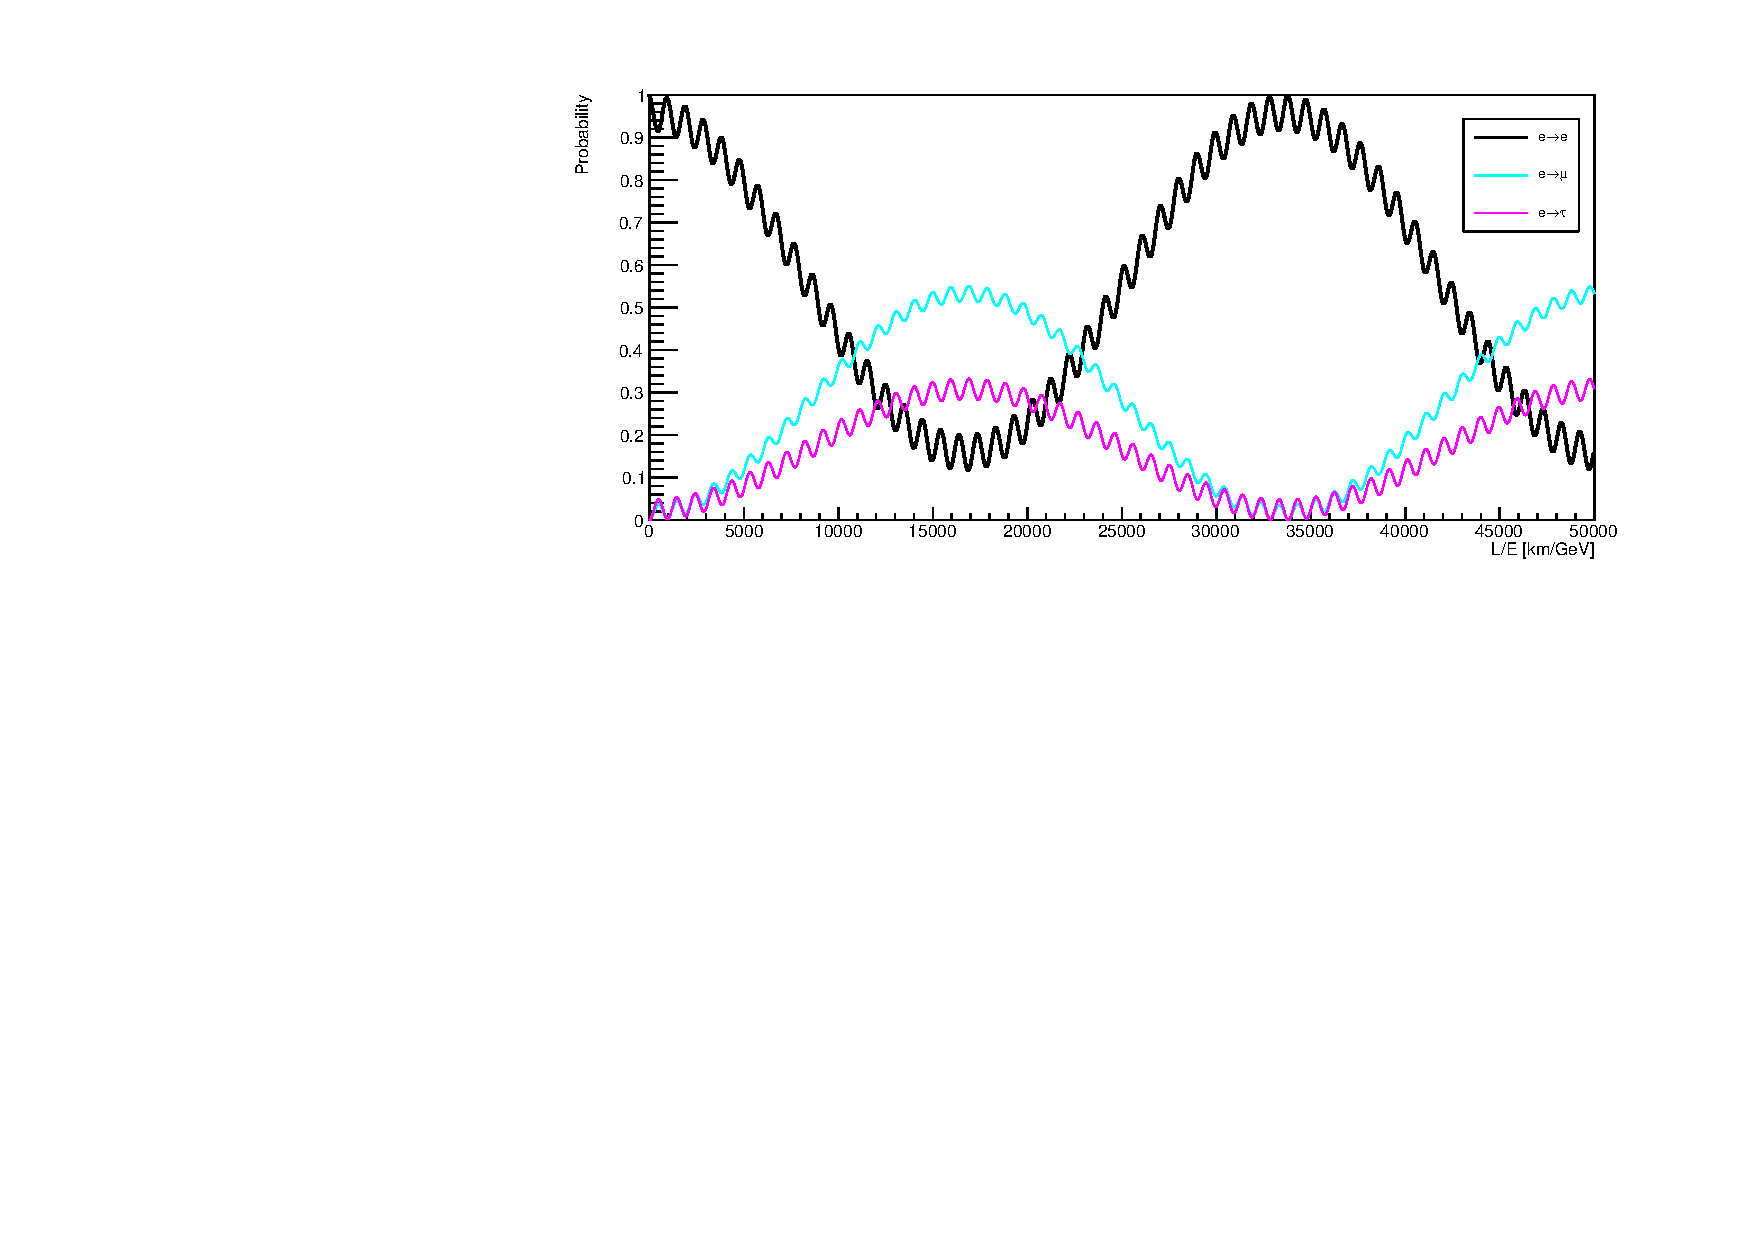
\includegraphics[width=0.95\linewidth]{Figures/Oscillation_2017Params_0CP.pdf}
\caption[Neutrino oscillation for an initial electron neutrino for 3 flavors of neutrino.]
{Neutrino oscillation for an initial electron neutrino for 3 flavors of neutrino.
This plot is generated via the latest parameters in \cite{Patrignani:2016xqp} assuming normal hierarchy. 
For this plot, $\delta_{CP}$ has been set to zero for illustrative purposes, but a value of 0 (or 2$\pi$) is disfavored at the 2.4$\sigma$ level.}
\label{fig:Oscillations_electron_long}
\end{figure}

Even with the latest data from neutrino oscillation experiments, the exact masses of the neutrinos cannot be determined.
This can be seen in \autoref{eq:OscillationProbability_2nu} where only the relative masses of the neutrinos play a role, not their absolute masses. 
Other data, however, can set limits on the absolute mass scale of the neutrinos.
Using data derived from the Cosmic Microwave Background and Baryon Acoustic Oscillations \cite{refId0}, the sum of the neutrino masses can be limited to, at 95\% C.L., $\sum_j m_j < 0.170~\textrm{eV}$, but there are existing models of neutrino mass generation where this result may not effectively constrain the neutrino mass \cite{Koksbang:2017rux} \cite{PhysRevLett.94.111801}.
Results from direct mass measurement experiments such as the Troitsk and Mainz experiments limit the electron antineutrino mass to, at 95\% C.L., $m_{\bar{\nu}_e} < 2.05~\textrm{eV}$ and $m_{\bar{\nu}_e} < 2.3~\textrm{eV}$, respectively \cite{Aseev:2011dq} \cite{Kraus:2004zw}, in a model-independent way.
Other upcoming experiments, KATRIN and Project 8, aim to measure these values with sensitivity up to 0.20 eV  and 0.04 eV, respectively \cite{Robertson:2013ziv} \cite{Esfahani:2017dmu}.

Another reason that \autoref{eq:OscillationProbability_2nu} is insensitive to the neutrino masses comes from the fact that the probabilities are unaffected by the sign of $\Delta m^2$.
However, this probability is for the propagation of a neutrino through vacuum, but in matter-dense regions, such as the sun, this probability is no longer correct.
This Mikheyev-Smirnov-Wolfenstein effect has been observed in solar neutrino measurements and allows for the determination that $\Delta m_{21}^2>0$ \cite{1367-2630-6-1-139}.
The sign of $\Delta m_{32}^2$ is still unknown, although long-baseline experiments of neutrino oscillation through the Earth aim to determine this effect.
Because of this, there are two possible scenarios for neutrino mass ordering, either $m_1 < m_2 < m_3$, called Normal Hierarchy (NH), or $m_3 < m_1 < m_2$, called Inverted Hierarchy (IH), shown in \autoref{fig:neutrinosfigs3nuspic}.
Recent results from the NOvA experiment point towards a NH Universe, but nothing yet to conclusively answer this question. \cite{Adamson:2017gxd}.
\begin{figure}[tbph]
\centering
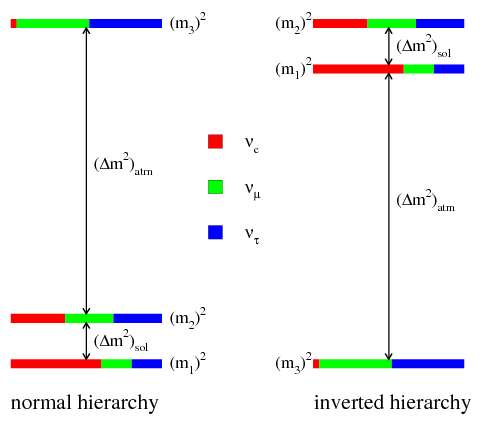
\includegraphics[width=0.8\linewidth]{Figures/Neutrinos_figs_3nuspic.png}
\caption[The mass orderings in both normal and inverted hierarchy.]
{The mass orderings in both normal and inverted hierarchy.
The sign of $(\Delta m^2)_{\textrm{atm}}$ is not known, which causes the difference between the two scenarios.
Figure from \cite{Hewett:2012ns}.}
\label{fig:neutrinosfigs3nuspic}
\end{figure}

\subsection{Dirac and Majorana Masses}
\label{ssec:Dirac and Majorana Masses}

With the mass of neutrinos shown to be non-zero, the Standard Model can be extended to include the masses for the neutrinos, but this opens up another question for how exactly the neutrino mass comes in to the Standard Model Lagrangian.
For the other fundamental fermionic particles, e.g. the electron that has charge $\textrm{e}^-$, the corresponding antiparticle will have the opposite charge, e.g. the positron with charge $\textrm{e}^+$ charge.
This, therefore, means that the particle and antiparticle are distinct particles.
The neutrino is unique in this regard as it is the only electrically neutral fundamental fermion, meaning the neutrino may be identical to its own antiparticle.
Fermions that are not identical to their own antiparticles, e.g. electrons and up quarks, are called Dirac fermions, while fermions that are identical to their own antiparticles are called Majorana fermions.
These two types of fermions have their masses arise in different ways in the Standard Model.

A particle with a Dirac mass appears in the Standard Model Lagrangian as
\begin{align}
&= -m(\bar{\psi_L}\psi_R + \bar{\psi_R}\psi_L) \\
&= -m\bar{\psi_L}\psi_R + h.c.,
\label{eq:DiracMass_chiral}
\end{align}
after decomposing the spinor, $\psi$, into its left- and right-handed chiral states.
In order to make the above expressions clearer by taking the assumption that a particle's mass is derived purely from the Dirac term, the field is given by
\begin{equation}
\psi = \psi_L + \psi_R,
\end{equation}
\autoref{eq:DiracMass_chiral} can be rewritten as
\begin{align}
\mathcal{L} &= -m\bar{\psi}\psi. \label{eq:DiracMass}
\end{align}

For a Majorana particle, the mass term does not couple between left- and right-handed chiral states and appears solely as single-handed fields $\psi_L$ and the charge conjugate $\psi_L^c$ as follows,
\begin{align}
\mathcal{L}_L &= -\frac{1}{2}m_L\bar{\psi^c_L}\psi_L+h.c. \label{eq:MajoranaMass_chiral} \\
\mathcal{L}_R &= -\frac{1}{2}m_R\bar{\psi^c_R}\psi_R+h.c.
\end{align}
What can be seen from \autoref{eq:DiracMass} and \autoref{eq:MajoranaMass_chiral} is that when the term in \autoref{eq:DiracMass} acts on a particle $\psi$, it leaves the particle as a $\psi$, but when the term in \autoref{eq:MajoranaMass_chiral} acts on a particle $\psi$, it converts the particle into its antiparticle $\bar{\psi}$.
If we assign a `lepton number' of $+1$ for particles and $-1$ for antiparticles, then the Dirac mass term conserves lepton number while the Majorana mass term does not.

However, a particle need not be purely Dirac or Majorana. In general, a particle can have both mass terms due to other interactions such as the seesaw mechanism described in \autoref{sssec:Seesaw Mechanism}. In this case, the Lagrangian contains both the Dirac and Majorana terms as follows:
\begin{align}
\mathcal{L} = & -\frac{1}{2}m_D(\bar{\psi}_L\psi_R+\bar{\psi}^c_L\psi^c_R)+m_L\bar{\psi}_L\psi^c_R+m_R\bar{\psi}^c_L\psi_R +h.c. \\
\mathcal{L} = &\frac{1}{2} \begin{pmatrix}
\bar{\psi}_L,& \bar{\psi}^c_L \\
\end{pmatrix} \begin{pmatrix}
m_L & m_D \\
m_D & m_R
\end{pmatrix}
\begin{pmatrix}
\psi^c_R \\
\psi_R
\end{pmatrix}.
\label{eq:DiracAndMajoranaMass}
\end{align}

\subsubsection{Seesaw Mechanisms}
\label{sssec:Seesaw Mechanism}
While \autoref{eq:DiracAndMajoranaMass} is a Lagrangian that accounts for both Dirac and Majorana masses, it is not immediately obvious from where this mechanism arises.
For example, the masses of the other particles in the Standard Model arise from the Higgs mechanism.
However, if the masses of the neutrinos were a result of the same Higgs mechanism as the other fermions, the Yukawa coupling between neutrinos and the Higgs would have to be a surprisingly small number, $\lesssim 10^{-11}$, so there should be some other mechanism that can explain the mass scale of the neutrinos \cite{Merle:2013gea}.
In addition, while the Standard Model can be modified to include neutrino oscillations, this addition does not offer any explanation of why the mass of the neutrino is of order $10^6$ times lighter than the electron, the next lightest known fundamental particle.
However, the addition of a Majorana nature for neutrinos could be the cause of this difference and explain the million times lower mass.
One of the simplest methods in which the observed mass of the neutrinos could be realized is known as the seesaw mechanism \cite{PhysRevD.22.2227}.
This name is derived from the fact that, in this model, the left-handed light neutrinos are balanced out by the existence of more massive particles.
There are two main types of models for this mechanism, called the type-I and type-II seesaw mechanisms.
In the type-I seesaw mechanism, shown in \autoref{fig:TypeISeesawMechanism}, the neutrino mass is generated through fermion exchange, e.g. with the addition of heavy right-handed neutrinos, and in the type-II mechanism, shown in \autoref{fig:TypeIISeesawMechanism}, scalar boson exchange generates the neutrino mass.
The model most commonly considered in the field of \zeronubb is the type-I seesaw mechanism and is discussed in greater detail in \autoref{sec:Neutrinoless Double Beta Decay}.
\begin{figure}[tbph]
\centering
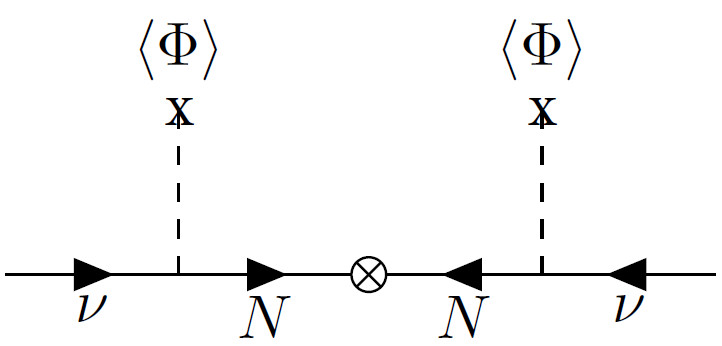
\includegraphics[width=0.40\linewidth]{Figures/TypeISeesaw.png}
\caption[Type-I seesaw mechanism]
{The type-I seesaw mechanism for neutrino mass generation wherein right-handed neutrinos, labelled $\textrm{N}$, contribute to the mass of the neutrinos.
Figure adapted from \cite{MIRANDA2016436}.}
\label{fig:TypeISeesawMechanism}
\end{figure}
The type-I seesaw mechanism with right-handed neutrinos then introduces a mass matrix for the neutrinos as follows:
\begin{equation}
M =\begin{pmatrix}
0 & m_D \\
m_D & M_R
\end{pmatrix}.
\end{equation}
If we take that the Dirac mass occurs for neutrinos in the same manner as for the other leptons in the Standard Model, i.e. due to electroweak symmetry breaking and the Higgs mechanism, then we can predict the value of the mass of the right-handed neutrinos.
In the case where $M_R \gg m_D$, the two neutrino masses become $M_R$ and $\frac{m_D^2}{M_R}$.
Taking $m_D$ to be $\approx1~\textrm{MeV}$, a meV-scale neutrino exists with a heavy right-handed neutrino of mass $10^{15}~\textrm{eV}$.

\begin{figure}[tbph]
    \centering
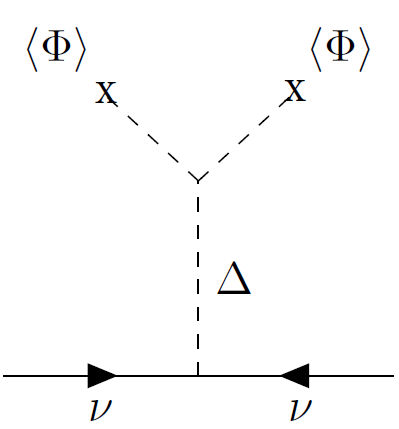
\includegraphics[width=0.40\linewidth]{Figures/TypeIISeesaw.png}
    \caption[Type-II seesaw mechanism.]
    {The type-II seesaw mechanism for neutrino mass generation wherein a boson, labelled $\Delta$, contributes to the mass of the neutrinos.
    Figure adapted from \cite{MIRANDA2016436}.}
    \label{fig:TypeIISeesawMechanism}
\end{figure}


\section{Baryogenesis}
If the neutrino is demonstrated to have a Majorana mass, there are possible far-reaching implications to the evolution of the early universe.
In particular, after the Big Bang, matter and antimatter should have been produced in equal amounts; however, the matter in the universe has won out over the antimatter, evidenced by measurements of the observable universe showing that is is purely matter on large scales.
For example, if there were antimatter galaxies or sectors of the universe, we would be able to observe large releases of energy due to matter-antimatter annihilation from collisions of galaxies or if there were an antimatter-dominated region of the universe due to annihilations at the border between the matter and antimatter regions.
This implies that the universe has a preference for slightly more baryons than antibaryons \cite{Canetti:2012zc}.
The requirements for a process to create this asymmetry are summed up in the Sakharov conditions for baryogenesis \cite{Sakharov:1967dj}:
\begin{enumerate}
\item Baryon number, B, violation
\item Charge, C, and Charge Parity, CP, violation
\item Interactions out of thermal equilibrium
\end{enumerate}
The first condition is needed so that there is a physics process within which a baryon can be created or an anti-baryon destroyed.
Assigning baryons such as protons and neutrons $\textrm{B}=1$, antibaryons $\textrm{B}=-1$, and non-baryonic matter $\textrm{B}=0$, this constraint can be written as $\Delta \textrm{B}\neq0$.
On its own, baryon number violation is not enough to create an imbalance between matter and antimatter as a process that has $\Delta\textrm{B}\neq0$ could just be reversed and prevent an asymmetry from forming.
Therefore, the second condition requires that a process with $\Delta\textrm{B}\neq0$ occurs more often for baryon creation or anti-baryon destruction than the reverse, i.e., $\Gamma(\Delta \textrm{B}>1) > \Gamma(\Delta \textrm{B}<-1)$.
Finally, the third condition requires that the process has to occur when the universe is not in thermal equilibrium as other processes would have to oppose whatever process satisfies the first two Sakharov conditions due to CPT (charge, parity, and time reversal) symmetry.

Therefore, in order to determine what caused the universe to evolve from equal parts matter and antimatter into the matter-dominated universe we see today, processes which satisfy all three Sakharov conditions are needed. In the framework of the Standard Model, Baryon number is not a fundamental symmetry such as electric charge and is merely an ``accidental" symmetry of the Lagrangian without an associated mediator like the photon.
While baryon number cannot be violated classically in the Standard Model Lagrangian, quantum effects, viz. sphaleron processes, may violate it \cite{PhysRevLett.37.8} \cite{KUZMIN198536}, and, while these effects satisfy the other two Sakharov conditions, do not have enough of an effect to explain the measured asymmetry,
\begin{align}
\Delta &= \frac{N_B - N_{\bar{B}}} {N_B + N_{\bar{B}}} \biggr\rvert_{T \gtrsim 1~\textrm{GeV}},
\label{eq:BAU_earlyuniverse}
\end{align}
where $N_B$ and $N_{\bar{B}}$ are the number of baryons and anti-baryons, respectively, when the asymmetry formed with the universe at a temperature of approximately 1 GeV.
This Baryon Asymmetry in the Universe (BAU) can be inferred from the current abundance of baryons and photons in the universe at the current temperature of 0.2 meV.
In this way, \autoref{eq:BAU_earlyuniverse} can be written as
\begin{align}
    \Delta &\sim \eta = \frac{N_B}{N_\gamma} \biggr\rvert_{T = 0.2 meV}
    \label{eq:eta_lateuniverse}
\end{align}
as the main product of baryon-antibaryon annihilation are photons, given by $N_\gamma$, and the number of anti-baryons remaining in the universe is vanishingly small.
Calculations from fitting parameters due to Big Bang Nucleosynthesis from the abundance of light elements in the intergalactic medium and calculations from the Cosmic Microwave Background data both give values of $\eta\sim 10^{-10}$ \cite{Canetti:2012zc}.
However, the contributions to $\eta$ from Standard Model processes predict an $\eta$ of $10^{-20}$, far below the observed value.

\subsection{Majorana Neutrinos and Leptogenesis}
However, these sphaleron processes conserve another symmetry, viz. $\textrm{B}-\textrm{L}$, where L is the lepton number and has similar rules to the baryon number described above.
Therefore, a place to look for baryon number violation may be in the lepton sector.
In this case, the imbalance between matter and antimatter is due to an imbalance in leptons that transfers over to the baryons.
This `leptogenesis' would have to fulfill an analogous set of Sakharov conditions to that described above.
This violation is possible if the neutrino is its own antiparticle, for example, in the interaction $d + d \rightarrow u + u + e + e$ in \autoref{fig:0nuBB}, lepton number is violated by $\Delta\textrm{L}=2$.
\begin{figure}[tbph]
\centering
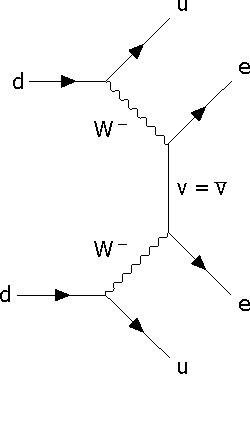
\includegraphics[width=0.35\linewidth]{Figures/0NuBB_clip.pdf}
\caption[The Feynman diagram for a lepton-number violating process.]
{The Feynman diagram for a lepton-number violating process.
Two down quarks convert to up quarks and emit a $\textrm{W}^{-}$ boson which exchange a neutrino and emit an electron.
This process is possible only if the neutrino is its own antiparticle.}
\label{fig:0nuBB}
\end{figure}
This method of lepton number violation would then also be associated with a baryon number violating process with $\Delta\textrm{B}=2$ as well.
To make this scenario of leptogenesis even more attractive as a candidate for baryon number asymmetry, the quantum effects that violate baryon number are unsuppressed at the high temperatures of the early universe.
Therefore, this lepton number violation could transfer to the baryon sector and result in the matter-dominated observable universe seen today.